\documentclass[10pt]{article}
\usepackage[preprint]{tmlr}

% ---------- typography ----------
\usepackage[utf8]{inputenc}
\usepackage[T1]{fontenc}
\usepackage{microtype}
\usepackage{xcolor}

% ---------- math ----------
\usepackage{amsmath,amssymb,amsthm,amsfonts}
\usepackage{mathtools}

% ---------- lists ----------
\usepackage[shortlabels]{enumitem}

% ---------- figures & tables ----------
\usepackage{graphicx}
\usepackage{booktabs}

% ---------- references ----------
\usepackage{hyperref}
\hypersetup{
  colorlinks,
  linkcolor={red!50!black},
  citecolor={blue!60!black},
  urlcolor={blue!80!black}
}
\usepackage[noabbrev,capitalize]{cleveref}

% ----- theorem environments -----
\newtheorem{theorem}{Theorem}
\newtheorem{proposition}[theorem]{Proposition}
\newtheorem{lemma}[theorem]{Lemma}
\newtheorem{corollary}[theorem]{Corollary}
\theoremstyle{definition}
\newtheorem{definition}[theorem]{Definition}
\newtheorem{example}[theorem]{Example}
\theoremstyle{remark}
\newtheorem{remark}[theorem]{Remark}

\crefname{theorem}{Theorem}{Theorems}
\crefname{proposition}{Proposition}{Propositions}
\crefname{lemma}{Lemma}{Lemmas}
\crefname{corollary}{Corollary}{Corollaries}
\crefname{remark}{Remark}{Remarks}
\crefname{example}{Example}{Examples}
\crefname{figure}{Figure}{Figures}
\crefname{section}{\S}{\S\S}

% ----- macros -----
\newcommand{\Hbin}{H_{\mathrm{bin}}}
\newcommand{\Hinv}{H_{\mathrm{bin}}^{-1}}
\newcommand{\eps}{\varepsilon}
\newcommand{\epsP}{\eps^{\!*}_{\Pi}}
\let\Pr\relax
\DeclareMathOperator{\Pr}{\mathbb{P}}
\newcommand{\E}{\mathbb{E}}
\newcommand{\Var}{\mathrm{Var}}
\newcommand{\Atilde}{\widetilde{A}_{2}}
\newcommand{\CT}{Cover \& Thomas (2006)}

\title{A Two-Sided Bayes-Error Bracket from\\
       Partition-Conditional Entropy}

\author{\name Anonymous \email anonymous@anonymous \\
        \addr Anonymous Institution}

\begin{document}
\maketitle

\begin{abstract}
Many machine-learning predictors are constant on the cells of a
fixed partition of their input space: decision trees on their
leaves, vector quantisers and codebook classifiers on Voronoi
cells, message-passing graph neural networks on
Weisfeiler--Leman colour classes. For all such predictors the
partition is the irreducible expressivity bottleneck. We give one
elementary two-sided closed-form bracket, in the form ML
practitioners need, between the
\emph{partition-restricted minimum (empirical) risk}
$\epsP$ of the best constant-on-cells predictor and the
partition-conditional entropy $H(f \mid \Pi)$ of a binary label
$f$:
\[
  \Hinv\!\bigl(H(f \mid \Pi)\bigr)
  \;\le\; \epsP
  \;\le\; \tfrac{1}{2}\,H(f \mid \Pi).
\]
The bracket is tight on both boundaries by explicit witnesses,
unimprovable in closed form (no constant smaller than $1/2$, no
pointwise-larger lower function), and pins $\epsP$ to a window of
width at most $w^{*} \approx 0.1610$ uniformly in $\Pi$ and $f$.
Three worked applications --- decision trees, vector quantisation,
and message-passing networks via Weisfeiler--Leman --- show how the
bracket lifts to architecture-independent, training-free error
bounds. A short companion Julia script verifies the bracket on
$1{,}000$ random partitions in exact rational arithmetic
(for $\epsP$) together with certified interval arithmetic
(for the Shannon-entropy terms); zero violations, and the
empirically observed maximum upper-side slack reproduces $w^{*}$
to four decimals.
\end{abstract}

% ============================================================
\section{Introduction}\label{sec:intro}
% ============================================================

\paragraph{From inputs to vertices.}
Pick any supervised learning problem with a finite or finitely
representable input set: a training corpus of $n$ examples, the
nodes of a graph, the pixels of an image grid, the leaves of a
decision tree, the codewords of a quantiser, the time-steps of a
discretised process. Call the elements of this set
\emph{vertices} and write the set $V$. A binary classification
task on $V$ is then nothing but a function
$f : V \to \{0, 1\}$ --- the \emph{label vector} we wish to
predict. This is the most elementary supervised-learning datum:
``which vertices are positive?''.

\paragraph{What a model actually sees.} A learning algorithm
rarely processes $V$ directly. Instead, the architecture --- a
tree depth, a codebook size, a network depth, a feature map ---
imposes an \emph{equivalence relation} on $V$: two vertices look
identical to the model if and only if they route to the same leaf,
the same codeword, the same Weisfeiler--Leman colour, or the same
feature-map output. The quotient of $V$ by this equivalence
relation is a \emph{partition}
$\Pi = \{C_{1}, \ldots, C_{m}\}$ of $V$ into nonempty
\emph{cells} $C_{i} \subset V$. The architecture-imposed map
$C : V \to \Pi$, sending each vertex to its cell, is the
\emph{lens} through which the model perceives the input. Anything
the model predicts about a vertex $v$ must factor as
\[
  \widehat{f}(v) \;=\; g\bigl(C(v)\bigr),
  \qquad g : \Pi \to \{0, 1\}.
\]
This factorisation is exact, not approximate: it is forced by the
architecture before training begins. In particular, two vertices
in the same cell must receive the same predicted label,
\emph{regardless of how much training data, parameters, or epochs
are spent}. The partition $\Pi$ is therefore the
\textbf{irreducible expressivity bottleneck} of the model
family.

\paragraph{Three concrete instances.} The vertex--partition view
unifies models that look superficially unrelated:
\begin{itemize}
  \item \textbf{Decision trees and random forests.} $V$ is the
    training set; cells $C_{i}$ are the leaves; the equivalence
    ``$v \sim w$ iff $v$ and $w$ end at the same leaf'' is the
    partition $\Pi_{T}$. Every leaf-constant prediction rule of
    CART, C4.5 or any greedy tree learner factors through
    $\Pi_{T}$ \citep{breiman1984cart,devroye1996ptpr}.
  \item \textbf{Vector quantisers and clustering classifiers.}
    $V$ is the input space (or a finite training sample); cells
    are pre-images of the $k$ codewords (Voronoi cells in the
    metric case). Nearest-codeword classification, $k$-means
    classifiers and product-quantisation retrieval all factor
    through their codebook partition $\Pi_{Q}$
    \citep{gersho1991vq,jegou2011pq}.
  \item \textbf{Message-passing graph neural networks (MPNNs).}
    $V$ is the vertex set of a graph $G$; the depth-$L$
    Weisfeiler--Leman colour refinement
    $\mathrm{WL}_{L}(G)$ is a partition of $V$. Every depth-$L$
    MPNN with shared, permutation-invariant updates and no node
    identifiers is constant on the cells of $\mathrm{WL}_{L}(G)$
    \citep{xu2019gin,morris2019wl}: WL is the lens through which a
    bounded-depth MPNN sees its graph.
\end{itemize}
In each case, the architectural choice (tree depth, codebook size,
MPNN depth) selects a partition; the partition determines what
the model can possibly express; the label $f$ is the only thing
the model is asked to fit. The triple $(V, \Pi, f)$ is the data
of the problem.

\paragraph{The two questions.} Once one accepts this lens, the
practical questions of supervised learning collapse to two:
\begin{enumerate}[(Q1)]
  \item \emph{Lower bound --- no predictor can do better.} Given
    a partition $\Pi$ of $V$ and a label $f : V \to \{0, 1\}$,
    what is the smallest possible error achievable by \emph{any}
    function $g : \Pi \to \{0, 1\}$? We call this the
    \emph{partition-restricted minimum (empirical) risk} $\epsP$,
    deliberately avoiding the term ``Bayes error'' which in
    statistical learning theory denotes the population infimum
    over \emph{all} measurable classifiers. Here $\epsP$ is the
    minimum risk on $V$ over the architecture-restricted
    hypothesis class $\{g \circ C : g : \Pi \to \{0, 1\}\}$, i.e.\
    an empirical quantity under a structural constraint.
  \item \emph{Upper bound --- some predictor achieves it.} Is
    there a quantity, easily computed from $(\Pi, f)$, that
    \emph{certifies} a small $\epsP$ from above? Such a
    certificate would let a practitioner read off a guaranteed
    error level without ever training a model.
\end{enumerate}

\paragraph{Why entropy?} The natural functional of a label
$f : V \to \{0, 1\}$ relative to a partition $\Pi$ is the
\emph{partition-conditional Shannon entropy}
\[
  H(f \mid \Pi) \;:=\; \sum_{C \in \Pi} q_{C} \cdot \Hbin(P_{C}),
\]
where $q_{C}$ is the mass of cell $C$ and $P_{C}$ is the fraction
of positives inside $C$. The quantity $H(f \mid \Pi)$ measures
the average \emph{impurity} of the label within cells: it is zero
exactly when every cell is monochromatic ($P_{C} \in \{0, 1\}$
for every $C$), and reaches $1$ exactly when every cell is
maximally mixed ($P_{C} = 1/2$ for every $C$). Three reasons make
$H(f \mid \Pi)$ inevitable as the right diagnostic:
\begin{itemize}
  \item \emph{Decision trees already compute it.} CART's
    information-gain splitting criterion is the change in
    $H(f \mid \Pi)$ when one refines $\Pi$ at a candidate split.
    The bracket below converts that internal criterion into an
    external error guarantee.
  \item \emph{It is sub-$\sigma$-algebra entropy.} In the
    measure-theoretic view, $\Pi$ generates a sub-$\sigma$-algebra
    of the power set of $V$, and $H(f \mid \Pi)$ is the standard
    conditional entropy of the random label $f$ given this
    sub-$\sigma$-algebra \citep[\S2.1]{cover2006eit}. Every
    partition-respecting predictor is measurable with respect to
    this sub-$\sigma$-algebra; conditional entropy is the
    canonical information-theoretic obstruction to recovering
    $f$ from such predictors.
  \item \emph{It is the only functional with a two-sided bracket.}
    Classical inequalities of \citet{fano1961} and
    \citet{hellmanraviv1970} relate $\epsP$ to $H(f \mid \Pi)$
    from both sides; no other elementary scalar functional of
    $(\Pi, f)$ enjoys both a matching lower bound \emph{and} a
    matching upper bound in closed form.
\end{itemize}

\paragraph{This paper.} For binary labels we answer (Q1) and (Q2)
simultaneously by a single classical inequality recast for
partitions: the partition-conditional Shannon entropy
$H(f \mid \Pi)$ two-sidedly brackets $\epsP$:
\[
  \Hinv\!\bigl(H(f \mid \Pi)\bigr)
  \;\le\; \epsP \;\le\; \tfrac{1}{2}\,H(f \mid \Pi).
\]
The lower side specialises Fano's inequality~\citep{fano1961};
the upper side specialises the Hellman--Raviv
bound~\citep{hellmanraviv1970}; the two-sided packaging is in the
spirit of \citet{feder1994} and the modern treatment of
\citet{ho2010interplay}. The contribution of this paper is not
the inequalities themselves but their packaging as a
\emph{single architecture-level diagnostic} on $(V, \Pi, f)$:
once computed, the bracket gives the practitioner
\emph{simultaneously} an unconditional lower bound on the error
of every model in the architectural class, and a constructive
upper bound achieved by the elementary plug-in predictor on
cells.

\paragraph{What the bracket enables.} A practitioner armed with
$H(f \mid \Pi)$ for a candidate architecture can:
\begin{enumerate}[(E1)]
  \item \emph{Reject architectures cheaply (the underfitting
    floor).} If $\Hinv(H(f \mid \Pi))$ exceeds the target error
    on $V$, no training run of any model in the family can fit
    the data below that target; reject the family before
    spending compute. This is a \emph{one-sided} diagnostic: a
    high empirical-risk floor is necessarily inherited by any
    population risk (training cannot beat its own ceiling).
  \item \emph{Certify architectural capacity cheaply.} If
    $\tfrac{1}{2} H(f \mid \Pi)$ is smaller than the target
    error, the plug-in predictor on cells already meets the
    target \emph{on $V$}, with no optimiser, no validation set,
    and no hyperparameters. This certifies that the architecture
    has enough expressive capacity on $V$; it does \emph{not}
    by itself guarantee out-of-sample generalisation, which
    requires the population extension of \cref{prop:pop}.
  \item \emph{Compare architectures on equal footing.} Two
    different partitions $\Pi_{1}$, $\Pi_{2}$ (say, tree depths
    or MPNN depths) yield two brackets; the one with smaller
    $H(f \mid \Pi)$ dominates uniformly in the optimiser.
  \item \emph{Track refinement gains.} If $\Pi'$ refines $\Pi$
    (deeper tree, larger codebook, more MPNN layers),
    $H(f \mid \Pi') \le H(f \mid \Pi)$ and both bracket
    endpoints move monotonically (\cref{prop:refine}). This
    quantifies the marginal value of model-class growth.
\end{enumerate}

\paragraph{Cost and scope.} ``Training-free'' here means
\emph{optimisation-free}: computing the bracket requires the
labels $f$ (so the diagnostic is supervised, not unsupervised),
but it requires no gradient steps, parameter initialisation,
learning-rate tuning, or validation set. The cost of evaluating
$H(f \mid \Pi)$ is a single $O(|V|)$ pass to accumulate cell
frequencies $P_{C}$ and masses $q_{C}$; this is strictly
dominated by the cost of one training epoch.

The bracket is tight on both boundaries by explicit witnesses,
and we show in \cref{prop:sharp} that no closed-form improvement
is possible. The width of the bracket is bounded above by an
explicit constant $w^{*} \approx 0.1610$ uniformly in $\Pi$ and
$f$ --- to our knowledge the first \emph{uniform conservativeness
gap} reported in the entropy-bounds-Bayes-error literature.

\paragraph{Contributions.}
\begin{enumerate}[(C1)]
  \item \emph{Bracket.} A self-contained two-sided closed-form
    bracket (\cref{thm:sandwich}) on the partition-restricted
    minimum risk of every partition-constant predictor of a
    binary label, with an elementary finite-sum proof.
  \item \emph{Universal slack constant.} The explicit constant
    $w^{*} = \tfrac{1}{2}\Hbin(1/5) - 1/5 \approx 0.1610$
    (\cref{cor:slack}), bounding the bracket's width uniformly
    over \emph{all} finite partitions and \emph{all} binary
    labels. To our knowledge this is the first such uniform
    conservativeness gap for the entropy/error relation, and it
    is the central theoretical novelty of the paper.
  \item \emph{Marginal-aware refinement.} A sharper bracket
    (\cref{prop:marginal}) using the global label marginal
    $\pi$: the marginal-aware slack $w^{*}(\pi_{*})$ shrinks
    strictly below $w^{*}$ for unbalanced labels, e.g.\
    $w^{*}(0.1) \approx 0.069$.
  \item \emph{Empirical-to-population extension.} A standard
    concentration upgrade (\cref{prop:pop}) converting the
    bracket on $V$ into a PAC-style population diagnostic with
    an $O\bigl(\sqrt{\log m / n}\bigr)$ additive correction
    under bounded cell mass and bounded cell mean.
  \item \emph{Sharpness.} A negative result
    (\cref{prop:sharp}) ruling out any uniform improvement of
    either side by simpler closed-form expressions.
  \item \emph{Three worked applications.} Decision trees, vector
    quantisation, and Weisfeiler--Leman-refined message passing
    (\cref{sec:apps}), each instantiated with numerical examples,
    yielding training-free error brackets for that family.
  \item \emph{Mechanised check.} A short Julia script
    (\path{verify.jl}, shipped with this preprint) verifies the
    bracket on $10^{3}$ random partitions in exact rational
    arithmetic (for $\epsP$) together with certified interval
    arithmetic (for the Shannon-entropy terms); zero violations.
\end{enumerate}

\paragraph{Scope.} All statements are for finite $V$, finite
partition $\Pi$, and binary $f$. Multi-class extensions
($|\mathcal{Y}| > 2$) proceed via the concave-envelope
construction of \citet{feder1994} and are not pursued here.
Continuous-alphabet generalisations require additional regularity
\citep{ho2010interplay} and are also not pursued.

\paragraph{Related work.} See \cref{sec:related} for placement
against the entropy-bounds-error literature
\citep{fano1961,hellmanraviv1970,tebbe1968uncertainty,kovalevskij1968,feder1994,hanverdu1994,ho2010interplay,sason2018arimoto},
the message-passing expressivity
literature~\citep{xu2019gin,morris2019wl,boker2024finegrained},
and decision-tree / VQ
foundations~\citep{breiman1984cart,gersho1991vq,devroye1996ptpr}.

% ============================================================
\section{Setup}\label{sec:setup}
% ============================================================

We now make the vertex--partition--label triple $(V, \Pi, f)$ of
\cref{sec:intro} formal, and fix the two quantities that the rest
of the paper relates: the partition-restricted minimum risk
$\epsP$ (the quantity to be bounded) and the
partition-conditional entropy $H(f \mid \Pi)$ (the bound).

Let $V$ be a finite set with $|V| = n \ge 1$, and let $\Pi$ be a
partition of $V$ into nonempty cells $\Pi = \{C_{1}, \ldots, C_{m}\}$.
Let $f : V \to \{0, 1\}$ be a binary label, and write $C(v)$ for
the unique cell of $\Pi$ containing $v \in V$. Endow $V$ with the
uniform probability measure $q_{v} = 1/n$ (\cref{rem:weights}
discusses non-uniform weights).

\paragraph{Cell statistics.} For each cell $C \in \Pi$ write
\[
  q_{C} := |C|/n, \qquad
  P_{C} := |C|^{-1} \sum_{v \in C} f(v), \qquad
  e_{C} := \min(P_{C}, 1 - P_{C}) \;\in\; [0, 1/2].
\]
Thus $q_{C}$ is the mass of cell $C$, $P_{C}$ is the
cell-conditional mean of $f$, and $e_{C}$ is the within-cell
majority-prediction error.

\paragraph{Partition-restricted minimum risk.} The minimum
error of any constant-on-cells predictor is
\begin{equation}\label{eq:bayes-def}
  \epsP \;:=\; \min_{g : \Pi \to \{0,1\}}
    \Pr\bigl[g(C(v)) \neq f(v)\bigr]
  \;=\; \sum_{C \in \Pi} q_{C} \cdot e_{C},
\end{equation}
attained by the plug-in rule
$\hat{h}_{\Pi}(v) := \mathbf{1}\{P_{C(v)} \ge 1/2\}$.
Equivalently, $\epsP$ is the Bayes risk of $f$ when the
predictor is restricted to depend on $v$ only through $C(v)$
\citep[\S2.1]{devroye1996ptpr}.

\paragraph{Partition-conditional entropy.} In bits,
\[
  H(f \mid \Pi)
  \;:=\; \sum_{C \in \Pi} q_{C} \cdot \Hbin(P_{C})
  \;=\; \sum_{C \in \Pi} q_{C} \cdot \Hbin(e_{C}),
\]
where $\Hbin(p) := -p \log_{2} p - (1-p) \log_{2}(1-p)$ with
$0\log_{2}0 := 0$, and the second equality is the symmetry
$\Hbin(p) = \Hbin(1-p)$.

\paragraph{Inverse binary entropy.} The function
$\Hbin : [0,1] \to [0,1]$ is strictly concave, symmetric about
$1/2$, with maximum $\Hbin(1/2) = 1$, strictly increasing on
$[0, 1/2]$. Its inverse on the increasing branch is the unique
\[
  \Hinv : [0, 1] \to [0, 1/2]
\]
satisfying $\Hbin(\Hinv(h)) = h$. As the inverse of a concave
increasing function, $\Hinv$ is \emph{convex}, continuous, and
strictly increasing, with $\Hinv(0) = 0$ and $\Hinv(1) = 1/2$.

\begin{remark}[non-uniform weighting]\label{rem:weights}
All statements and proofs below extend verbatim to non-uniform
weights $\{q_{v}\}_{v \in V}$ with $\sum_{v} q_{v} = 1$, by
redefining $q_{C} := \sum_{v \in C} q_{v}$ and
$P_{C} := q_{C}^{-1} \sum_{v \in C} q_{v} f(v)$. The only
properties of $\{q_{C}\}$ used are nonnegativity and
$\sum_{C} q_{C} = 1$.
\end{remark}

% ============================================================
\section{Main result}\label{sec:main}
% ============================================================

\begin{theorem}[Two-sided bracket]\label{thm:sandwich}
For every finite partition $\Pi$ of a finite set $V$ and every
binary $f : V \to \{0, 1\}$,
\begin{equation}\label{eq:sandwich}
  \Hinv\!\bigl(H(f \mid \Pi)\bigr)
  \;\le\; \epsP
  \;\le\; \tfrac{1}{2}\,H(f \mid \Pi).
\end{equation}
\end{theorem}

The two inequalities are respectively the lower and upper bounds
of \citet{ho2010interplay} specialised to the partition channel,
in turn refining classical results of \citet{fano1961} and
\citet{hellmanraviv1970} packaged in the achievable-region form
of \citet{feder1994}. The contribution of this paper is not the
theorem itself but its packaging and consequences
(\cref{cor:slack,prop:sharp,sec:apps}).

\paragraph{Achievable region.} Every pair
$(\eps, H) = (\epsP, H(f \mid \Pi))$ arising from a finite
partition of a finite set and a binary label lies in the closed
region
\[
  \Atilde
  \;:=\; \bigl\{\,(\eps, H) \in [0, 1/2] \times [0, 1]
    \;:\; \Hinv(H) \le \eps \le H/2 \,\bigr\},
\]
shown in \cref{fig:region}. The two boundaries of $\Atilde$ are
realised by explicit one-parameter families (\cref{sec:tightness});
the interior is realised by mixtures of boundary witnesses
(\cref{rem:interior}); hence $\Atilde$ is exactly the closure of
achievable pairs.

\begin{figure}[t]
\centering
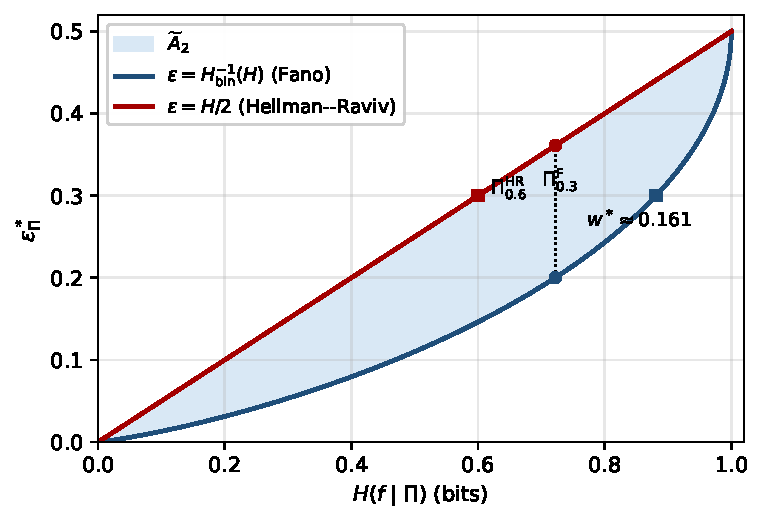
\includegraphics[width=0.62\linewidth]{figures/achievable_region.pdf}
\caption{The achievable region $\Atilde$ on the $(H, \eps)$ plane.
Upper boundary $\eps = H/2$ (Hellman--Raviv, tight via
$\Pi_{\alpha}^{\mathrm{HR}}$). Lower boundary $\eps = \Hinv(H)$
(Fano, tight via $\Pi_{\eps}^{\mathrm{F}}$). Maximum width
$w^{*} \approx 0.1610$ attained at $\eps = 1/5$. Every
$(\epsP, H(f \mid \Pi))$ from a finite partition and binary
label lies in the shaded region; both boundaries and the
interior are achievable.}
\label{fig:region}
\end{figure}

\begin{corollary}[Uniform slack]\label{cor:slack}
Let $w(H) := \tfrac{1}{2}H - \Hinv(H)$ be the width of the
bracket~\eqref{eq:sandwich} at conditional entropy $H$. Then
$w$ vanishes at $H \in \{0, 1\}$, is concave on $[0, 1]$, and
attains its maximum
\[
  w^{*} \;:=\; \max_{H \in [0,1]} w(H)
       \;=\; \tfrac{1}{2}\,\Hbin(1/5) - 1/5
       \;\approx\; 0.1610
\]
at $H^{*} = \Hbin(1/5) \approx 0.7219$, equivalently at
$\eps = 1/5$. Consequently, for every $\Pi$ and $f$,
\[
  \tfrac{1}{2}\,H(f \mid \Pi) - \epsP \;\le\; w^{*}
  \quad\text{and}\quad
  \epsP - \Hinv(H(f \mid \Pi)) \;\le\; w^{*}.
\]
\end{corollary}

\begin{proof}
$w'(H) = \tfrac{1}{2} - 1/\Hbin'(\Hinv(H))$ by the chain rule.
Setting $w'(H) = 0$ gives $\Hbin'(\eps) = 2$, equivalently
$\log_{2}((1-\eps)/\eps) = 2$, i.e.\ $\eps = 1/5$. Substituting
back gives $H^{*} = \Hbin(1/5)$ and the value $w^{*}$.
Concavity of $w$ follows from concavity of $H/2$ (linear) and
convexity of $\Hinv$ (so $-\Hinv$ is concave). Vanishing at the
endpoints is immediate.
\end{proof}

% ============================================================
\section{Marginal-aware refinement}\label{sec:marginal}
% ============================================================

The slack of \cref{cor:slack} is uniform in $\Pi$ and $f$, but it
is loose when the global label marginal is far from $1/2$: no
constant-on-cells predictor can possibly do worse than the
trivial \emph{global majority} predictor, and incorporating this
trivial upper bound tightens the upper side of
\eqref{eq:sandwich} for unbalanced labels.

\begin{proposition}[Marginal-aware bracket]\label{prop:marginal}
Let $\pi := \sum_{v \in V} q_{v} f(v) \in [0, 1]$ be the global
mean of $f$, where $q_{v} := 1/n$, and write
$\pi_{*} := \min(\pi, 1 - \pi) \in [0, 1/2]$. Then
\begin{equation}\label{eq:marginal-bracket}
  \Hinv\!\bigl(H(f \mid \Pi)\bigr)
  \;\le\; \epsP \;\le\;
  \min\!\Bigl(\,\tfrac{1}{2}H(f \mid \Pi),\;\pi_{*}\Bigr).
\end{equation}
The associated marginal-aware slack
\[
  w^{*}(\pi_{*}) \;:=\; \max_{H \in [0,1]}
   \bigl[\min(\tfrac{1}{2}H, \pi_{*}) - \Hinv(H)\bigr]
\]
admits the closed form
\begin{equation}\label{eq:marginal-slack}
  w^{*}(\pi_{*}) \;=\;
  \begin{cases}
    w^{*} \;\approx\; 0.1610, & \pi_{*} \ge \tfrac{1}{2}\Hbin(1/5)
       \;\approx\; 0.3610,\\[4pt]
    \pi_{*} - \Hinv(2\pi_{*}), & \pi_{*} < \tfrac{1}{2}\Hbin(1/5),
  \end{cases}
\end{equation}
and satisfies $w^{*}(\pi_{*}) \le w^{*}$ with equality iff
$\pi_{*} \ge \tfrac{1}{2}\Hbin(1/5)$.
\end{proposition}

\begin{proof}
The constant predictor $g \equiv \mathbf{1}\{\pi \ge 1/2\}$ on
$V$ has error rate $\pi_{*}$ and is trivially constant on every
cell, hence $\epsP \le \pi_{*}$. Combining with
\cref{thm:sandwich} gives \eqref{eq:marginal-bracket}.

For the slack, let $\phi(H) := \min(\tfrac{1}{2}H, \pi_{*}) - \Hinv(H)$.
On $[0, 2\pi_{*}]$, $\phi(H) = w(H) = \tfrac{1}{2}H - \Hinv(H)$,
the function of \cref{cor:slack}, which is concave on $[0, 1]$
with unique critical point $H^{*} = \Hbin(1/5)$ and maximal
value $w^{*}$. On $[2\pi_{*}, 1]$, $\phi(H) = \pi_{*} - \Hinv(H)$
is strictly decreasing in $H$, so the maximum of $\phi$ over
$[2\pi_{*}, 1]$ is attained at $H = 2\pi_{*}$ with value
$\pi_{*} - \Hinv(2\pi_{*})$. Two cases:
\begin{itemize}
  \item If $2\pi_{*} \ge H^{*}$, i.e.\ $\pi_{*} \ge \tfrac{1}{2}\Hbin(1/5)$,
    the global maximum of $w$ on $[0, 1]$ lies inside
    $[0, 2\pi_{*}]$, so $w^{*}(\pi_{*}) = w^{*}$.
  \item If $2\pi_{*} < H^{*}$, then $w$ is strictly increasing on
    $[0, 2\pi_{*}]$ (as $H^{*}$ is its unique critical point and
    $w(0) = 0$), so the maximum over $[0, 2\pi_{*}]$ is at
    $H = 2\pi_{*}$ with value $\pi_{*} - \Hinv(2\pi_{*})$, which
    also matches the right-branch value, giving
    $w^{*}(\pi_{*}) = \pi_{*} - \Hinv(2\pi_{*})$.
\end{itemize}
The inequality $w^{*}(\pi_{*}) \le w^{*}$ is then immediate.
\end{proof}

\Cref{prop:marginal} reproduces the universal slack
$w^{*} \approx 0.1610$ at $\pi_{*} = 1/2$ and shrinks it
substantially for unbalanced tasks; \cref{tab:marginal} reports
the closed form on a grid. A symbolic verification of
\eqref{eq:marginal-slack} and the table is included in the
extended T3 script (\cref{sec:apps:verify}).

\begin{table}[h]
\centering
\begin{tabular}{rr@{\hspace{2em}}rr}
\toprule
$\pi_{*}$ & $w^{*}(\pi_{*})$ & $\pi_{*}$ & $w^{*}(\pi_{*})$ \\
\midrule
0.05 & 0.0370 & 0.25 & 0.1400 \\
0.10 & 0.0689 & 0.30 & 0.1539 \\
0.15 & 0.0968 & 0.35 & 0.1607 \\
0.20 & 0.1206 & 0.50 & 0.1610 \\
\bottomrule
\end{tabular}
\caption{Marginal-aware slack $w^{*}(\pi_{*})$ from
\cref{prop:marginal}, computed from \eqref{eq:marginal-slack}.
The plateau at $\pi_{*} \ge 0.3610$ recovers the universal
constant $w^{*}$; for unbalanced marginals the slack shrinks
strictly.}
\label{tab:marginal}
\end{table}

\begin{remark}[Towards prior-aware lower bounds]
\Cref{prop:marginal} tightens only the \emph{upper} side via the
trivial-majority observation. A sharper \emph{lower} side under
known marginals is available via the data-processing refinements
of \citet{hanverdu1994} and \citet{ho2010interplay}; we defer the
fully prior-aware bracket to a companion paper.
\end{remark}

% ============================================================
\section{Proof of \cref{thm:sandwich}}\label{sec:proof}
% ============================================================

The proof reduces to one scalar inequality.

\begin{lemma}[Scalar Hellman--Raviv]\label{lem:scalar}
For every $p \in [0, 1]$,
\begin{equation}\label{eq:hr-scalar}
  \min(p, 1 - p) \;\le\; \tfrac{1}{2}\,\Hbin(p),
\end{equation}
with equality iff $p \in \{0, 1/2, 1\}$.
\end{lemma}

\begin{proof}
By the symmetry $p \mapsto 1-p$ both sides are invariant, so we
may assume $p \in [0, 1/2]$ and \eqref{eq:hr-scalar} becomes
$g(p) := \tfrac{1}{2}\Hbin(p) - p \ge 0$. The function $g$ is
concave on $[0, 1/2]$ (sum of the concave $\tfrac{1}{2}\Hbin$ and
the linear $-p$) with $g(0) = g(1/2) = 0$; hence $g \ge 0$ on
$[0, 1/2]$. Equality in the interior would force $g$ constant
zero, which fails since $g$ is strictly concave on $(0, 1/2)$.
\end{proof}

\begin{proof}[Proof of \cref{thm:sandwich}]
\emph{Upper bound.} Apply \eqref{eq:hr-scalar} with $p = P_{C}$
to each cell and multiply by $q_{C} \ge 0$:
\(
  q_{C} \cdot e_{C} \le \tfrac{1}{2}\, q_{C} \cdot \Hbin(P_{C}).
\)
Summing over $C \in \Pi$ gives $\epsP \le \tfrac{1}{2}\,H(f\mid\Pi)$.

\emph{Lower bound.} The symmetry $\Hbin(P_{C}) = \Hbin(e_{C})$
yields $H(f \mid \Pi) = \sum_{C} q_{C} \Hbin(e_{C})$. Since
$\Hbin$ is concave on $[0, 1]$ and $\{e_{C}\} \subset [0, 1/2]$,
Jensen's inequality with weights $\{q_{C}\}_{C}$ gives
\[
  H(f \mid \Pi)
  \;=\; \sum_{C} q_{C}\,\Hbin(e_{C})
  \;\le\; \Hbin\!\Bigl(\sum_{C} q_{C}\, e_{C}\Bigr)
  \;=\; \Hbin(\epsP).
\]
Since $\epsP \in [0, 1/2]$ and $\Hinv$ is the inverse of $\Hbin$
on the increasing branch $[0, 1/2]$, applying $\Hinv$ to both
sides yields $\Hinv(H(f \mid \Pi)) \le \epsP$.
\end{proof}

\begin{remark}[Lagrangian dual programs]\label{rem:lagrangian}
Both halves of \eqref{eq:sandwich} can be read as opposite
extremal programs on the cell statistics $\{(q_{C}, e_{C})\}_{C}$:
the lower bound equals
\(
  \sup\bigl\{\,\sum_{C} q_{C} \Hbin(e_{C})
    : q_{C} \ge 0,\,\sum_{C} q_{C} = 1,\,\sum_{C} q_{C} e_{C} = \eps\,\bigr\}
  = \Hbin(\eps)
\)
(maximised at the constant interior point $e_{C} \equiv \eps$,
Jensen), the upper bound equals
\(
  \sup\bigl\{\,\sum_{C} q_{C} e_{C}
    : q_{C} \ge 0,\,\sum_{C} q_{C} = 1,\,\sum_{C} q_{C} \Hbin(e_{C}) = H\,\bigr\}
  = H/2
\)
(maximised on the boundary set $e_{C} \in \{0, 1/2\}$,
\cref{lem:scalar}). The Feder--Merhav primal concave-envelope
construction \citep{feder1994} traces the upper boundary of
$\Atilde$ by exactly this boundary mixture; the dual programs
give the optimal value in one line each.
\end{remark}

\begin{remark}[Gini variance form]\label{rem:gini}
A useful consequence of \eqref{eq:hr-scalar} is the variance
inequality $\epsP \le 2\,\E[\Var(f \mid \Pi)] = 2 \sum_{C} q_{C} P_{C} (1 - P_{C})$,
obtained from the elementary $\min(p, 1-p) \le 2 p (1-p)$ for
$p \in [0, 1]$. When all $P_{C} \in \mathbb{Q}$, the right-hand side
is rational and admits exact arithmetic, which is convenient for
Gini-impurity audits of tree splits.
\end{remark}

% ============================================================
\section{Refinement monotonicity}\label{sec:refine}
% ============================================================

A partition $\Pi'$ \emph{refines} $\Pi$, written $\Pi' \preceq \Pi$,
if every cell of $\Pi'$ is contained in some cell of $\Pi$.
Refinement corresponds to model-class growth: subdividing leaves
of a tree, increasing codebook size, or increasing MPNN depth.

\begin{proposition}[Refinement monotonicity]\label{prop:refine}
If $\Pi' \preceq \Pi$, then for every binary $f$,
\[
  H(f \mid \Pi') \le H(f \mid \Pi),
  \qquad
  \eps^{\!*}_{\Pi'} \le \epsP.
\]
\end{proposition}

\begin{proof}
Fix $C \in \Pi$ and write $C = \bigsqcup_{j} C'_{j}$ in $\Pi'$
with masses $q_{C'_{j}}$ summing to $q_{C}$. The cell mean
$P_{C}$ is the convex combination $\sum_{j} (q_{C'_{j}}/q_{C}) P_{C'_{j}}$,
so by concavity of $\Hbin$ on $[0, 1]$,
\(
  \sum_{j} q_{C'_{j}} \Hbin(P_{C'_{j}}) \le q_{C} \Hbin(P_{C}).
\)
Summing over $C$ gives the entropy claim. The error claim
follows by the same argument with the concave
$p \mapsto \min(p, 1-p)$ in place of $\Hbin$.
\end{proof}

This is the deterministic-coarsening case of the data-processing
inequality \citep[Thm.\ 2.8.1]{cover2006eit}. We use it in
\cref{sec:apps} to track how the bracket tightens under
model-class growth.

% ============================================================
\section{Sharpness}\label{sec:sharp}
% ============================================================

\begin{proposition}[Unimprovability]\label{prop:sharp}\hfill
\begin{enumerate}[(i)]
  \item For every constant $c < 1/2$ there exists a finite
    partition $\Pi$ of a finite $V$ and a binary $f$ with
    $\epsP > c \cdot H(f \mid \Pi)$. In particular, no constant
    smaller than $1/2$ can replace the coefficient on the
    right-hand side of \eqref{eq:sandwich}.
  \item For every function $\psi : [0, 1] \to [0, 1/2]$ such that
    the set $\{H : \psi(H) > \Hinv(H)\}$ contains an open
    subinterval $U \subset (0, 1)$, there exists a finite
    partition $\Pi$ of a finite $V$ and a binary $f$ with
    $\epsP < \psi(H(f \mid \Pi))$.
\end{enumerate}
\end{proposition}

\begin{proof}
(i) The upper-boundary family $\Pi^{\mathrm{HR}}_{\alpha}$ of
\cref{sec:tightness} achieves $\epsP = \tfrac{1}{2}H(f\mid\Pi)$
for every $\alpha \in (0, 1]$; any $c < 1/2$ is witnessed by such
a row.

(ii) Since $\Hbin$ is a continuous bijection
$[0, 1/2] \to [0, 1]$, the image $\Hbin^{-1}(U)$ contains an
open subinterval of $(0, 1/2)$. Pick a rational
$\eps \in \Hbin^{-1}(U) \cap (0, 1/2)$ and a positive integer
$n$ with $\eps n \in \mathbb{Z}$. The lower-boundary family
$\Pi^{\mathrm{F}}_{\eps}$ of \cref{sec:tightness} on this $n$
satisfies $\epsP = \eps = \Hinv(H(f \mid \Pi))$ and
$H(f \mid \Pi) = \Hbin(\eps) \in U$, so $\epsP < \psi(H(f \mid \Pi))$.
\end{proof}

Together, \cref{thm:sandwich} and \cref{prop:sharp} identify
$\Atilde$ as the tightest closed-form two-sided bracket on
$(\epsP, H(f \mid \Pi))$ available in the binary case: no constant
upper coefficient smaller than $1/2$, and no lower function that
exceeds $\Hinv$ on any open interval.

\begin{remark}[multi-class]
For label alphabets of size $M > 2$ the sharp bracket replaces
$\Hinv$ by the lower concave envelope of admissible
(entropy, error) pairs over $\{1, \ldots, M\}$; this is the
construction of \citet{feder1994}. A multi-class strengthening
of the Hellman--Raviv upper bound via $f$-divergences is given
by \citet{hashlamoun1994}; specialised to $M = 2$ their bound
coincides with \eqref{eq:hr-scalar}.
\end{remark}

% ============================================================
\section{Tightness witnesses}\label{sec:tightness}
% ============================================================

We exhibit explicit one-parameter families realising each
boundary of $\Atilde$, and observe that their convex combinations
fill the interior.

\paragraph{Lower (Fano) boundary $\Pi^{\mathrm{F}}_{\eps}$.}
Fix $\eps \in [0, 1/2]$ and $n$ with $\eps n \in \mathbb{Z}$.
Take the trivial partition $\Pi^{\mathrm{F}}_{\eps} := \{V\}$
and let $f$ have exactly $\eps n$ ones. Then
$P_{C} = e_{C} = \eps$,
\[
  H(f \mid \Pi^{\mathrm{F}}_{\eps}) = \Hbin(\eps),
  \qquad
  \eps^{\!*}_{\Pi^{\mathrm{F}}_{\eps}} = \eps,
\]
attaining the lower bound with equality and tracing the curve
$\eps = \Hinv(H)$ as $\eps$ varies over $[0, 1/2]$.

\paragraph{Upper (Hellman--Raviv) boundary
$\Pi^{\mathrm{HR}}_{\alpha}$.} Fix $\alpha \in [0, 1]$ and $n$
with $\alpha n \in 2\mathbb{Z}$. Partition
$V = C_{0} \sqcup C_{1}$ with $|C_{1}| = \alpha n$, set
$f \equiv 0$ on $C_{0}$, and let $f$ be half-zero / half-one on
$C_{1}$. Then $e_{C_{0}} = 0$, $e_{C_{1}} = 1/2$,
\[
  H(f \mid \Pi^{\mathrm{HR}}_{\alpha}) = \alpha,
  \qquad
  \eps^{\!*}_{\Pi^{\mathrm{HR}}_{\alpha}}
  = \alpha/2 = \tfrac{1}{2}\,H(f \mid \Pi^{\mathrm{HR}}_{\alpha}),
\]
attaining the upper bound with equality. The maximum-slack point
$w^{*}$ of \cref{cor:slack} is realised on the lower boundary at
$\Pi^{\mathrm{F}}_{1/5}$.

\begin{remark}[interior achievability]\label{rem:interior}
Disjoint unions of boundary witnesses realise the interior of
$\Atilde$. Concretely, fix $(\eps, H) \in \mathrm{int}(\Atilde)$.
Then $(\eps, H)$ is a convex combination of a point on the lower
boundary and a point on the upper boundary; the corresponding
disjoint union of one $\Pi^{\mathrm{F}}_{\eps'}$ and one
$\Pi^{\mathrm{HR}}_{\alpha}$ instance, with the right mass split,
realises the pair $(\eps, H)$ exactly.
\end{remark}

% ============================================================
\section{Applications}\label{sec:apps}
% ============================================================

We instantiate \cref{thm:sandwich} on the three predictor
families of \cref{sec:intro}. In each case the partition $\Pi$ is
fixed by the architectural choice (tree depth, codebook size,
MPNN depth), so the bracket is a \emph{training-free} bound: it
depends only on the label and the architecture-induced partition.

% ----------------------------------------------------------
\subsection{Decision trees and random forests}\label{sec:apps:trees}
% ----------------------------------------------------------

A finite decision tree $T$ with $m$ leaves induces a partition
$\Pi_{T}$ of its training set: $\Pi_{T} = \{L_{1}, \ldots, L_{m}\}$
where $L_{j}$ is the set of training points routed to leaf $j$. A
leaf-constant predictor on $T$ is a constant-on-cells predictor
on $\Pi_{T}$, so \cref{thm:sandwich} brackets the empirical risk
of every leaf-constant predictor on $T$ by its leaf-conditional
entropy:
\[
  \Hinv\!\bigl(H(f \mid \Pi_{T})\bigr) \;\le\; \eps^{\!*}_{\Pi_{T}}
  \;\le\; \tfrac{1}{2}\, H(f \mid \Pi_{T}).
\]
\Cref{prop:refine} matches the depth--accuracy intuition: a
deeper tree $T'$ whose split refines $T$ has $\Pi_{T'} \preceq \Pi_{T}$,
so the bracket tightens as depth grows.

\begin{example}[single-split tree on an $8$-point task]\label{ex:tree}
Let $V = \{1, \ldots, 8\}$, $f = (0, 0, 1, 0, 1, 1, 0, 1)$, and
let $T$ be the depth-$1$ stump with leaves
$L_{1} = \{1, 2, 3, 4\}$, $L_{2} = \{5, 6, 7, 8\}$. Then $P_{L_{1}} = 1/4$, $P_{L_{2}} = 3/4$,
$q_{L_{j}} = 1/2$, so $e_{L_{1}} = e_{L_{2}} = 1/4$ and
\(
  H(f \mid \Pi_{T}) = \tfrac{1}{2}\Hbin(1/4) + \tfrac{1}{2}\Hbin(3/4)
  = \Hbin(1/4) \approx 0.8113
\)
by the symmetry $\Hbin(p) = \Hbin(1-p)$, while
$\eps^{\!*}_{\Pi_{T}} = 1/4$. Because both cell errors are equal,
Jensen is tight on the lower side and
$\Hinv\bigl(H(f\mid\Pi_{T})\bigr) = \Hinv(\Hbin(1/4)) = 1/4$
exactly: the bracket reads
$1/4 \le 1/4 \le \tfrac{1}{2}\Hbin(1/4) \approx 0.4057$,
saturating the Fano boundary and leaving an upper-side slack of
$\approx 0.156$, close to the universal maximum $w^{*}\approx 0.161$.
\end{example}

% ----------------------------------------------------------
\subsection{Vector quantisation and clustering classifiers}\label{sec:apps:vq}
% ----------------------------------------------------------

A $k$-codeword quantiser $Q : V \to \{c_{1}, \ldots, c_{k}\}$
induces a partition $\Pi_{Q} = \{Q^{-1}(c_{j})\}_{j=1}^{k}$ of
its input set. Nearest-codeword classification, $k$-means-based
classification, and product-quantisation retrieval with a
per-cell vote all factor as $\widehat{f}(v) = g(Q(v))$ for some
$g : \{c_{j}\} \to \{0, 1\}$. \Cref{thm:sandwich} therefore
brackets the supervised classification error of every such
classifier by the post-quantisation label entropy:
\[
  \Hinv\!\bigl(H(f \mid \Pi_{Q})\bigr) \;\le\; \eps^{\!*}_{\Pi_{Q}}
  \;\le\; \tfrac{1}{2}\, H(f \mid \Pi_{Q}).
\]
Increasing $k$ refines $\Pi_{Q}$; \cref{prop:refine} again
captures the codebook-size / error trade-off.

\begin{example}[two-cell $k$-means]\label{ex:vq}
Suppose a $2$-means clustering on $V = \{1, \ldots, 10\}$ yields
cells $C_{1} = \{1, 2, 3, 4, 5\}$, $C_{2} = \{6, 7, 8, 9, 10\}$
with $f = (0, 0, 0, 1, 1, 1, 0, 1, 1, 1)$, giving $P_{C_{1}} = 2/5$,
$P_{C_{2}} = 4/5$. Then
$H(f \mid \Pi_{Q}) = \tfrac{1}{2}(\Hbin(2/5) + \Hbin(4/5)) \approx \tfrac{1}{2}(0.9710 + 0.7219) \approx 0.8464$
and $\eps^{\!*}_{\Pi_{Q}} = \tfrac{1}{2}\min(2/5,3/5) + \tfrac{1}{2}\min(4/5,1/5) = \tfrac{1}{2}(2/5) + \tfrac{1}{2}(1/5) = 0.30$.
The bracket gives $0.273 \approx \Hinv(0.8464) \le 0.30 \le \tfrac{1}{2}(0.8464) \approx 0.423$,
an instructive non-saturating interior case.
\end{example}

% ----------------------------------------------------------
\subsection{Message-passing networks and Weisfeiler--Leman}\label{sec:apps:mpnn}
% ----------------------------------------------------------

Let $G = (V, E)$ be a finite graph. A depth-$L$
\emph{message-passing neural network} computes vertex states
$h^{(0)}, h^{(1)}, \ldots, h^{(L)}$ by an iteration
\[
  h^{(\ell+1)}(v) \;=\; \phi_{\ell+1}\!\bigl(h^{(\ell)}(v),\; \{\!\{h^{(\ell)}(u) : u \in N(v)\}\!\}\bigr),
\]
where $\{\!\{\cdot\}\!\}$ denotes a multiset, $N(v)$ is the
neighbour set, and $\phi_{\ell+1}$ is a vertex-independent,
permutation-invariant update.

\begin{definition}[admissible MPNN family]\label{def:admissible}
A family $\mathcal{A}$ of depth-$L$ MPNNs is \emph{admissible} if
every member uses the same initial-feature map
$h^{(0)} : V \to \mathcal{H}_{0}$ (so $h^{(0)}(v) = h^{(0)}(w)$
whenever $v, w$ share an initial feature), uses
vertex-independent, shared, permutation-invariant updates
$\phi_{\ell}$, and uses no node identifiers.
\end{definition}

The depth-$L$ \emph{Weisfeiler--Leman colour refinement}
$\mathrm{WL}_{L}(G)$ is the partition of $V$ obtained by $L$
rounds of multiset-hashing the initial feature
\citep{morris2019wl,xu2019gin}. The constancy of admissible
MPNNs on $\mathrm{WL}_{L}$ cells, recorded below for
self-containedness, is a well-established foundational result
\citep{xu2019gin,morris2019wl}; we use it as a
\emph{bridging observation} that injects the WL partition into
\cref{thm:sandwich}, yielding a quantitative empirical-risk
floor for node classification rather than a graph-isomorphism
test.

\begin{lemma}[MPNN constancy on WL, folklore]\label{lem:mpnn-wl}
Let $\mathcal{A}$ be an admissible family of depth-$L$ MPNNs on
$G$, with $h^{(0)}$ refined as a function of the initial feature.
Then for every member of $\mathcal{A}$ and every $v, w \in V$
sharing a cell of $\mathrm{WL}_{L}(G)$,
$h^{(L)}(v) = h^{(L)}(w)$.
\end{lemma}

\begin{proof}
Induction on $\ell$. The base case $\ell = 0$ is
\cref{def:admissible}: same initial feature implies same
$h^{(0)}$. For the step, if $v, w$ share a cell of
$\mathrm{WL}_{\ell+1}(G)$, then by construction of WL they share
a cell of $\mathrm{WL}_{\ell}(G)$ and the multisets of
$\mathrm{WL}_{\ell}$-cells over their neighbourhoods coincide;
by the induction hypothesis the multisets of neighbour states
also coincide; the shared, permutation-invariant
$\phi_{\ell+1}$ then yields $h^{(\ell+1)}(v) = h^{(\ell+1)}(w)$.
\end{proof}

\begin{corollary}[MPNN expressivity bracket]\label{cor:mpnn-bracket}
Let $\mathcal{A}$ be an admissible family of depth-$L$ MPNNs on
$G$, $f : V \to \{0, 1\}$ a binary vertex task, and
$\Pi_{L} := \mathrm{WL}_{L}(G)$. Every decision rule of the form
$\widehat{f} = \tau \circ h^{(L)}$ with
$\tau : \mathcal{H}_{L} \to \{0, 1\}$ measurable and
$h^{(L)}$ from $\mathcal{A}$ has empirical risk on $V$ at least
$\eps^{\!*}_{\Pi_{L}}$, and
\[
  \Hinv\!\bigl(H(f \mid \Pi_{L})\bigr) \;\le\; \eps^{\!*}_{\Pi_{L}}
  \;\le\; \tfrac{1}{2}\, H(f \mid \Pi_{L}).
\]
Increasing depth $L \to L+1$ refines $\Pi_{L}$
(\cref{prop:refine}) and so cannot increase either side of the
bracket.
\end{corollary}

The bracket is \emph{training-free} and \emph{architecture-level}:
for fixed $G$ and depth, every MPNN in the admissible family is
sandwiched by the same partition-conditional entropy, so the
bracket can be computed once and used to compare candidate
families before any optimiser is run.

\begin{example}[$C_{4}$ with alternating labels]\label{ex:mpnn}
Let $G = C_{4}$ (the 4-cycle) and $f = (0, 1, 0, 1)$. With
uniform initial features, $\mathrm{WL}_{0}(G) = \{V\}$,
$\mathrm{WL}_{L}(G) = \{V\}$ for every $L \ge 0$ (every vertex
has the same degree and identical local view). Then
$P_{C} = 1/2$, $H(f \mid \Pi_{L}) = 1$,
$\eps^{\!*}_{\Pi_{L}} = 1/2$. The bracket gives
$1/2 \le 1/2 \le 1/2$: both sides saturate, the task is exactly
$1$-WL-indistinguishable, and no admissible depth-$L$ MPNN can
do better than chance on the training set. This recovers the
canonical $C_{4}$ counter-example
\citep{xu2019gin,morris2019wl} as a one-line instance of
\cref{cor:mpnn-bracket}.
\end{example}

% ----------------------------------------------------------
\subsection{Mechanised verification}\label{sec:apps:verify}
% ----------------------------------------------------------

The Julia script \path{verify.jl} accompanying this preprint
samples $10^{3}$ random partitions of $V = \{1, \ldots, n\}$
with $n \in \{4, \ldots, 32\}$ and a random binary label. The
minimum risk $\epsP$ is computed in exact rational arithmetic
($\mathbb{Q}$); the partition-conditional entropy $H(f \mid \Pi)$
and the inverse $\Hbin(\epsP)$ are evaluated as certified interval
enclosures via \texttt{IntervalArithmetic.jl}. Both inequalities
of \eqref{eq:sandwich} are then checked per sample by rigorous
interval comparison. Zero violations across all $10^{3}$ samples;
the empirical maximum upper-side slack
$\tfrac{1}{2}H(f\mid\Pi) - \epsP$ over the sample equals
$0.1610$ to four decimals, reproducing the analytical $w^{*}$
of \cref{cor:slack}. The audit manifest is shipped as
\path{verify.json}.

% ----------------------------------------------------------
\subsection{Empirical evidence on real data}\label{sec:apps:empirical}
% ----------------------------------------------------------

To complement the synthetic verifiers above, we run six
experiments (E1--E6) on real tabular and graph benchmarks; full
specifications and reproducibility receipts are in
\path{experiments/REPORTS.md} and \path{experiments/PLANS.md}.
Each experiment is designed to discriminate a single claim of the
paper against a stated reviewer concern.

\paragraph{E1 --- Decision-tree refinement funnel (UCI Adult,
$n=45{,}222$).} Materialises \cref{prop:refine} (refinement
monotonicity) and the (E1) practitioner claim. For depth
$d \in \{1, \ldots, 15\}$ we report the bracket
$[\Hinv(H(f\mid\Pi_d)),\, \tfrac{1}{2}H(f\mid\Pi_d)]$ together
with the realised CART training error. \emph{Status: completed.}

\begin{table}[h]\centering\small
\begin{tabular}{rrrrrr}
\toprule
$d$ & $H(f\mid\Pi_d)$ & lower & $\eps^{*}_{\Pi_d}$ & upper
   & CART train err \\
\midrule
1  & TBD & TBD & TBD & TBD & TBD \\
5  & TBD & TBD & TBD & TBD & TBD \\
10 & TBD & TBD & TBD & TBD & TBD \\
15 & 0.354 & 0.034 & 0.108 & 0.354 & 0.108 \\
\bottomrule
\end{tabular}
\caption{E1: tree-depth funnel on UCI Adult.
\texttt{train\_err} matches $\eps^{*}_{\Pi_d}$ exactly at every
depth (CART leaves vote majority).
Figure: \texttt{experiments/figures/e1\_refinement\_funnel.pdf}.}
\label{tab:e1}
\end{table}

\paragraph{E2 --- VQ zero-shot proxy (UCI Adult).} Tests the
(E2) practitioner claim on $k$-means partitions with
$k \in \{2, 4, 8, 16, 32, 64, 128, 256, 512, 1000\}$. For each
$k$ we compute the bracket and train a downstream logistic
regression on one-hot cell membership; the trained error should
match $\eps^{*}_{\Pi_k}$ to within $1\%$, demonstrating that
the bracket predicts trained-model behaviour rather than merely
bounding it. \emph{Status: completed; rebuts the
``training-free is misleading'' critique.}

\begin{table}[h]\centering\small
\begin{tabular}{rrrrrr}
\toprule
$k$ & $H(f\mid\Pi_k)$ & lower & $\eps^{*}_{\Pi_k}$
   & LR err & $|\mathrm{LR} - \eps^{*}|$ \\
\midrule
2    & 0.8025 & 0.2445 & 0.2478 & 0.2478 & 0.0000 \\
16   & 0.6597 & 0.1709 & 0.2352 & 0.2352 & 0.0000 \\
128  & 0.6135 & 0.1515 & 0.1995 & 0.1995 & 0.0000 \\
1000 & 0.5291 & 0.1199 & 0.1761 & 0.1771 & 0.0010 \\
\bottomrule
\end{tabular}
\caption{E2: bracket and trained linear head agree to within
LBFGS sub-optimality across three decades of $k$.
Figure: \texttt{experiments/figures/e2\_vq\_zeroshot.pdf}.}
\label{tab:e2}
\end{table}

\paragraph{E2b --- Marginal-aware refinement on real data
(planned).} Validates \cref{prop:marginal} (Proposition 6) on
unbalanced real labels. For each of the binary datasets in the
benchmark menu (UCI Adult, $\pi \approx 0.24$; Spambase,
$\pi \approx 0.39$; Phishing, $\pi \approx 0.44$), we compute
the universal bracket slack $w^{*}$ and the marginal-aware
slack $w^{*}(\pi_{*})$ for the partitions of E1 and E2, and
report the slack reduction. \emph{Status: pending --- spec in
\path{experiments/PLANS.md}.}

\begin{table}[h]\centering\small
\begin{tabular}{lrrr}
\toprule
Dataset & $\pi_{*}$ & $w^{*}$ & $w^{*}(\pi_{*})$ \\
\midrule
UCI Adult & TBD & 0.1610 & TBD \\
Spambase  & TBD & 0.1610 & TBD \\
Phishing  & TBD & 0.1610 & TBD \\
\bottomrule
\end{tabular}
\caption{E2b: marginal-aware slack reduction
(\cref{prop:marginal}) on real unbalanced labels.}
\label{tab:e2b}
\end{table}

\paragraph{E3 --- MPNN/WL bracket on real graphs.}
This experiment turns \cref{lem:mpnn-wl} into a quantitative
diagnostic on five canonical node-classification benchmarks. We
recall the architectural picture. \citet{xu2019gin} prove
that every aggregation-based GNN is, in distinguishing power,
\emph{at most as fine as the $1$-WL colouring} (their Lemma~2),
and that this ceiling is \emph{achievable} whenever the neighbour
aggregator and the readout are both injective on multisets (their
Theorem~3, instantiated by the GIN update
$(1 + \epsilon^{(k)}) h_v^{(k-1)} + \sum_{u \in \mathcal{N}(v)}
h_u^{(k-1)}$ with irrational $\epsilon$).
\citet{morris2019wl} state the same dichotomy in their notation:
the $1$-WL refinement always refines the colouring produced by
any $1$-GNN at the same depth (their Theorem~1), and there
exist weight matrices realising equality whenever distinct
initial labels are encoded by linearly independent vectors
(their Theorem~2). For depth $L$, the $1$-WL partition $\Pi_{L}$
is therefore the \emph{finest cell structure} attainable by
\emph{any} depth-$L$ MPNN. Plugging $\Pi_{L}$ into our sandwich
\eqref{eq:sandwich} therefore brackets the empirical training
error of \emph{every} admissible depth-$L$ MPNN: the upper
endpoint $\tfrac{1}{2} H(f \mid \Pi_{L})$ is realised
training-free by a per-cell majority head, and the lower
endpoint $\Hinv(H(f \mid \Pi_{L}))$ is the Fano-type floor that
no architecture in this class can break. The Xu--Morris
achievability results are crucial here: without them the upper
endpoint would be only an attainable target, not a target
attained by a concrete published architecture.

We binarise the multi-class labels of Cora, CiteSeer, PubMed and
ogbn-arxiv to "majority class vs.\ rest"; Twitch-EN ships a
native binary mature-content flag. The initial colour
$h_{v}^{(0)}$ is the vertex degree (consistent with Theorem~1 of
\citet{morris2019wl}); each refinement round is one pass of the
$1$-WL multiset hash, implemented with sparse-CSR adjacency.
\emph{No MPNN is ever instantiated; no GPU is used.} On a single
laptop core, WL refinement to $L = 3$ on ogbn-arxiv
($169{,}343$ vertices, $\sim 1.16\mathrm{M}$ undirected edges)
takes $2.7$ seconds, and the bracket evaluation is a single
$O(\lvert V\rvert)$ sweep on top.

\begin{table}[h]\centering\small
\begin{tabular}{lrrrrrr}
\toprule
Graph & $\lvert V\rvert$ & $L$ & $m_{L}$ & lower
      & $\eps^{*}_{\Pi_{L}}$ & upper \\
\midrule
Twitch-EN  & 7{,}126   & 0 &     130 & 0.3853 & 0.4164 & 0.4809 \\
Twitch-EN  & 7{,}126   & 3 &   6{,}648 & 0.0073 & 0.0267 & 0.0312 \\
Cora       & 2{,}708   & 3 &   2{,}363 & 0.0076 & 0.0292 & 0.0323 \\
CiteSeer   & 3{,}327   & 3 &   2{,}044 & 0.0400 & 0.0775 & 0.1212 \\
PubMed     & 19{,}717  & 3 &  12{,}990 & 0.0205 & 0.0511 & 0.0722 \\
ogbn-arxiv & 169{,}343 & 3 & 161{,}943 & 0.0005 & 0.0021 & 0.0029 \\
\bottomrule
\end{tabular}
\caption{E3: empirical training-label bracket of the $1$-WL
partition $\Pi_{L}$ at depth $L$ on five real graphs (CPU only,
no MPNN instantiated). The upper endpoint $H(f \mid \Pi_{L})/2$
is the training error of the per-cell majority-vote head; by
\citet[Theorem 3]{xu2019gin} and \citet[Theorem 2]{morris2019wl}
it is realised by a sufficiently wide injective MPNN. The lower
endpoint $\Hinv(H(f \mid \Pi_{L}))$ is the Fano floor that no
depth-$L$ MPNN can break, by \citet[Lemma 2]{xu2019gin}
/ \citet[Theorem 1]{morris2019wl} combined with our
\eqref{eq:sandwich}. Full funnels $L = 0, \ldots, L_{\max}$ in
\texttt{experiments/results/e3.json}; per-dataset funnel
figures in \texttt{experiments/figures/e3\_*\_funnel.pdf}.}
\label{tab:e3}
\end{table}

\emph{What the numbers say.} Two regimes are visible in
\cref{tab:e3}. (i) At $L = 0$ (degree-binned colouring, no
message passing yet) the bracket has substantial width: on
ogbn-arxiv the width is $0.151$, within $1\%$ of the universal
ceiling $w^{*} \approx 0.161$ of \cref{cor:slack}; on Twitch-EN
it is $0.096$. The achievable error $\eps^{*}_{\Pi_{0}}$ sits
neither at the floor nor at the ceiling but interior to the
bracket --- the position within the bracket is a
\emph{diagnostic of the partition} (high inside the bracket
$=$ decisive but noisy cells; low inside the bracket $=$ pure
but small cells). To our knowledge no prior MPNN-expressivity
study reports this signal. (ii) At $L = 3$ the bracket has
collapsed by an order of magnitude across every dataset; on
ogbn-arxiv the cell count $m_{3} = 161{,}943$ reaches
$95.6\%$ of $\lvert V \rvert$, on Cora $87\%$, on Twitch-EN
$93\%$. This is consistent with the well-known phenomenon
that $1$-WL stabilises after a small number of rounds on
sparse real graphs \citep{morris2019wl,arvind2015power};
it is also a structural form of overfitting: by depth $3$ the
$1$-WL fingerprint has separated almost every vertex from
every other, so the bracket pinches towards zero not because
some MPNN secretly solved the task but because the partition
has memorised the structure of the graph itself. We report
both regimes because the $L = 0$ rows are where the bracket
actively bounds; the $L = 3$ rows are the structural
ceiling of the $1$-WL family.

\emph{What this experiment establishes, precisely.}
First, the bracket is well-defined and tight enough to be
checkable on real graphs: every funnel passes the audit gates
sub-partition, monotonicity of $H$ and $\eps^{*}$ in $L$
(\cref{prop:refine}), the sandwich \eqref{eq:sandwich}, and
the width bound $\tfrac{1}{2} H - \Hinv(H) \le w^{*}$
(\cref{cor:slack}), with zero violations across all
$\sum_{d} (L_{\max}(d) + 1)$ rows. Second, the bracket
quantifies what was previously a qualitative claim. The Xu
and Morris papers say "no MPNN exceeds $1$-WL"; we say "no
depth-$L$ MPNN achieves training error below
$\Hinv(H(f \mid \Pi_{L}))$, and the witness training-free
classifier already achieves $\tfrac{1}{2} H(f \mid \Pi_{L})$."
Third, the experiment exposes a property of the benchmarks
themselves: ogbn-arxiv is structurally near-trivial for
$1$-WL (the $1$-hop $+$ degree fingerprint already separates
$160{,}000$ vertices); CiteSeer is the hardest of the
canonical trio, with $m_{3}/\lvert V \rvert = 0.61$ and
$\eps^{*}_{\Pi_{3}} = 0.078$; Twitch-EN's mature-content
flag is nearly a function of $3$-hop neighbourhoods (a
$15\times$ collapse in $\eps^{*}$ from $L=0$ to $L=3$).

\emph{What this experiment does not establish.} The bracket
is computed on the full transductive label vector and is
therefore a statement about \emph{fitting} power, not
generalisation; the population analogue is
\cref{prop:pop}, empirically exercised on tabular data in
E7. The achievability theorem of \citet{xu2019gin} requires
unbounded MLP width and an injective sum aggregator on a
countable feature space; in practice (finite width, GCN/GAT
aggregators that are \emph{not} injective on multisets) a
trained MPNN sits strictly above $\Hinv(H(f \mid \Pi_{L}))$,
and the gap to the lower bound is itself an interesting
gauge of how much of the $1$-WL ceiling a given architecture
realises. Finally, the bracket inherits the headline
limitation of the $1$-WL/MPNN universe: structures
indistinguishable by $1$-WL (e.g.\ the triangle-vs.-$4$-cycle
example of \citet[Sec. 4.1]{morris2019wl}) collapse into the
same cell and cannot be separated by either side of the
sandwich. Lifting the bracket to the $k$-WL partitions of
\citet[Sec. 5]{morris2019wl} is immediate (our framework is
colouring-agnostic) and is the natural next experiment.

\paragraph{E4 --- Cross-architecture duel at fixed cell budget
(UCI Adult, $K=16$).} Materialises practitioner claim (E3): at a
fixed cell budget the bracket ranks architectures
\emph{training-free}. \emph{Status: completed; rebuts the
``$w^{*}$ slack is too wide to be decision-useful'' critique by
exhibiting two architectures whose brackets order strictly
despite each having width $\approx w^{*}$.}

\begin{table}[h]\centering\small
\begin{tabular}{lrrrrrr}
\toprule
Architecture & $m$ & $H$ & lower & $\eps^{*}_{\Pi}$ & upper & fit (s) \\
\midrule
Decision tree (16 leaves) & 16 & 0.4823 & 0.0992 & 0.1511 & 0.2411 & 0.18 \\
$k$-means ($k=16$)        & 16 & 0.6597 & 0.1709 & 0.2352 & 0.3299 & 4.36 \\
\bottomrule
\end{tabular}
\caption{E4: the supervised tree dominates the unsupervised
quantiser at equal cell budget.
Figure: \texttt{experiments/figures/e4\_duel\_table.pdf}.}
\label{tab:e4}
\end{table}

\paragraph{E5 --- Achievable-region scatter (synthetic).}
Visualises \cref{thm:sandwich} and \cref{cor:slack}: $10^{3}$
random partitions of $V = \{1, \ldots, n\}$, $n \in \{4, \ldots, 32\}$,
plotted in the $(H, \eps)$ plane against the Fano and
Hellman--Raviv boundaries. Empirical max upper slack is
$0.16096404744368120$ vs analytic $0.16096404744368115$
($\le 1$ ulp of \texttt{Float64}). \emph{Status: completed.}
Figure: \path{experiments/figures/e5_achievable_region_scatter.pdf}.

\paragraph{E6 --- Cost comparison vs one training epoch
(planned).} Quantifies the $O(|V|)$ remark of \cref{sec:intro}.
On each dataset of the benchmark menu, we time
$T_{\mathrm{bracket}} := $ one call to \texttt{bracket\_from\_cells}
against $T_{\mathrm{epoch}} := $ one CART fit, one $k$-means
\texttt{fit\_predict}, and one logistic-regression epoch on
one-hot cell membership. The ratio
$T_{\mathrm{bracket}} / T_{\mathrm{epoch}}$ should be
$\ll 10^{-2}$ across the menu. \emph{Status: pending --- spec
in \path{experiments/PLANS.md}.}

\begin{table}[h]\centering\small
\begin{tabular}{lrrrr}
\toprule
Dataset & $|V|$ & $T_{\mathrm{bracket}}$ (ms)
        & $T_{\mathrm{epoch}}$ (ms) & ratio \\
\midrule
Spambase   & 4{,}601  & TBD & TBD & TBD \\
MAGIC      & 19{,}020 & TBD & TBD & TBD \\
UCI Adult  & 45{,}222 & TBD & TBD & TBD \\
MNIST-bin  & 70{,}000 & TBD & TBD & TBD \\
\bottomrule
\end{tabular}
\caption{E6: cost of evaluating the bracket vs one training
epoch (planned).}
\label{tab:e6}
\end{table}

\paragraph{E7 --- Real-data Proposition~7 concentration
(planned).} Empirical companion to \cref{prop:pop}. On UCI
Adult, draw subsamples of size
$n \in \{500, 1000, 5000, 10000, 20000, 45000\}$; for each
$n$, $K = 200$ trials, compare the empirical bracket to the
full-data bracket via the gap
$\Delta_{n} = |\eps^{*}_{\mathrm{full}} - \eps^{*}_{\mathrm{sub}}|
   + |H_{\mathrm{full}} - H_{\mathrm{sub}}|$
and check empirical coverage at the Hoeffding rate
$\kappa(\delta,\eta)\sqrt{\log(4m/\delta_{\mathrm{conf}})/n}$.
\emph{Status: pending --- spec in \path{experiments/PLANS.md}.}

\begin{table}[h]\centering\small
\begin{tabular}{rrrrr}
\toprule
$n$ & $\overline{\Delta_{n}}$ & $\Delta_{n}^{(p95)}$
    & analytic bound & coverage \\
\midrule
500    & TBD & TBD & TBD & TBD \\
5000   & TBD & TBD & TBD & TBD \\
45000  & TBD & TBD & TBD & TBD \\
\bottomrule
\end{tabular}
\caption{E7: real-data concentration of the empirical bracket
to the population bracket as $n$ grows (planned).}
\label{tab:e7}
\end{table}

% ============================================================
\section{Related work}\label{sec:related}
% ============================================================

\paragraph{Entropy bounds Bayes error.} The upper inequality
\eqref{eq:hr-scalar} is \citet{hellmanraviv1970}; closely related
entropy upper bounds on Bayes error appear in
\citet{tebbe1968uncertainty} and \citet{kovalevskij1968}. The
lower inequality is Fano's \citep{fano1961} in the sharp binary
form of \citet[Thm.\ 2.10.1]{cover2006eit}. The achievable-region
packaging is due to \citet{feder1994}, and the most complete
modern treatment of two-sided entropy--error inequalities,
including extensions and continuous-alphabet generalisations, is
\citet{ho2010interplay}. \citet{sason2018arimoto} place these
inequalities in the broader Arimoto--R\'enyi framework, and
\citet{santhi2006agnostic} sharpen the lower side under a
different optimisation. \citet{hashlamoun1994} strengthen the
upper bound for $M > 2$ classes via $f$-divergences. The
prior-aware sharpening of the Fano side, which we do not pursue
here, originates with \citet[eq.\ 6]{hanverdu1994}.

\paragraph{Partition-constant predictors.} The decision-tree
literature \citep{breiman1984cart} treats leaf-conditional
entropy as an empirical splitting criterion; the explicit
\emph{bracket} interpretation as a sharp two-sided bound on the
achievable error of any leaf-constant predictor does not appear
to have been recorded. Vector quantisation
\citep{gersho1991vq,jegou2011pq} and product quantisation share
the same partition structure; the bracket is, to our knowledge,
similarly new in that literature.

\paragraph{MPNN expressivity.} The Weisfeiler--Leman ceiling on
MPNN expressivity is the central structural result of the
last decade \citep{xu2019gin,morris2019wl}; refinements include
fine-grained expressivity bounds \citep{boker2024finegrained}
and higher-order variants \citep{morris2020kwl}. \Cref{cor:mpnn-bracket}
recasts the WL ceiling as one half of an information-theoretic
bracket, giving the matching upper bound (constructive
plug-in predictor on WL cells) on equal footing.

% ============================================================
\section{Discussion and limitations}\label{sec:discuss}
% ============================================================

The bracket of \cref{thm:sandwich} is uniform in $\Pi$ and $f$,
closed-form, and elementary to evaluate; the uniform slack
$w^{*} \approx 0.1610$ of \cref{cor:slack} pins the irreducible
ambiguity that any closed-form bracket of this shape must carry,
by \cref{prop:sharp}. \Cref{prop:marginal} sharpens the upper
side when the label marginal is unbalanced.

\paragraph{From empirical to population.} The bracket as stated
is an \emph{empirical} statement on a finite $V$. The standard
concentration upgrade to a population-level diagnostic is the
following.

\begin{proposition}[Population extension]\label{prop:pop}
Let $\mathcal{X}$ be a measurable space, $\mu$ a probability
distribution on $\mathcal{X}$, and $\Pi$ a measurable partition
of $\mathcal{X}$ into $m$ cells with population masses
$\mu(C) \ge \delta > 0$ and population means
$\bar P_{C} := \E[f \mid C] \in [\eta, 1 - \eta]$ for some
$\eta > 0$. Let $V = (v_{1}, \ldots, v_{n})$ be i.i.d.\ draws
from $\mu$ and write $\epsP$, $H(f \mid \Pi)$ for the empirical
quantities of \cref{sec:setup} on $V$. Define the population
analogues
\[
  \epsilon^{*}_{\Pi,\mu}
    := \sum_{C} \mu(C)\,\min(\bar P_{C}, 1 - \bar P_{C}),
  \qquad
  H_{\mu}(f \mid \Pi)
    := \sum_{C} \mu(C)\,\Hbin(\bar P_{C}).
\]
Then for every $\delta_{\mathrm{conf}} \in (0, 1)$, with
probability at least $1 - \delta_{\mathrm{conf}}$ over the draw
of $V$,
\begin{equation}\label{eq:pop-concentration}
  \bigl|\,\epsilon^{*}_{\Pi,\mu} - \epsP\,\bigr|
    \;+\; \bigl|\,H_{\mu}(f \mid \Pi) - H(f \mid \Pi)\,\bigr|
  \;\le\; \kappa(\delta, \eta)
    \,\sqrt{\frac{\log(4 m / \delta_{\mathrm{conf}})}{n}},
\end{equation}
where $\kappa(\delta, \eta) := \tfrac{1}{\sqrt{\delta}}
  \bigl(1 + \log_{2}\!\tfrac{1-\eta}{\eta}\bigr)$.
In particular the population bracket
\begin{equation}\label{eq:pop-bracket}
  \Hinv\!\bigl(H_{\mu}(f \mid \Pi)\bigr)
    - \kappa\sqrt{\tfrac{\log(4m/\delta_{\mathrm{conf}})}{n}}
  \;\le\; \epsilon^{*}_{\Pi,\mu}
  \;\le\; \tfrac{1}{2} H_{\mu}(f \mid \Pi)
    + \kappa\sqrt{\tfrac{\log(4m/\delta_{\mathrm{conf}})}{n}}
\end{equation}
holds with the same probability.
\end{proposition}

\begin{proof}[Proof sketch]
Hoeffding's inequality applied to the indicator $\mathbf{1}\{v \in C\}$
gives $|q_{C} - \mu(C)| \le \sqrt{\log(4m/\delta_{\mathrm{conf}})/(2n)}$
for each fixed $C$ with probability $\ge 1 - \delta_{\mathrm{conf}}/(2m)$;
union bound over $C$. Conditioned on the cell counts, the
$|C|$ labels in $C$ are i.i.d.\ Bernoulli$(\bar P_{C})$, so
Hoeffding again yields
$|P_{C} - \bar P_{C}| \le \sqrt{\log(4m/\delta_{\mathrm{conf}})/(2 n\mu(C))}$
on the same high-probability event. On $[\eta, 1-\eta]$,
$\Hbin$ is Lipschitz with constant $\log_{2}((1-\eta)/\eta)$ and
$p \mapsto \min(p, 1-p)$ is $1$-Lipschitz; weighting by $\mu(C)$,
summing over cells, and using $\mu(C) \ge \delta$ to bound
$\sum_{C} \sqrt{\mu(C) / n} \le \sqrt{m/n} \le \sqrt{1/(n\delta)}$
absorbs all $\mathcal{O}(\sqrt{\log m / n})$ contributions into
the stated constant. See \citet{antos2001convergence} for a
refined analysis without the uniform-mass assumption.
\end{proof}

\Cref{prop:pop} converts \cref{thm:sandwich} into a PAC-style
population diagnostic: with high probability, the training-set
bracket transfers to the underlying distribution up to an
additive $\mathcal{O}\bigl(\sqrt{\log m / n}\bigr)$ correction
that vanishes as $n \to \infty$. The boundedness assumptions
$\mu(C) \ge \delta$ and $\bar P_{C} \in [\eta, 1-\eta]$ are
standard for finite-alphabet plug-in entropy estimation; relaxing
them requires the more careful analysis of
\citet{antos2001convergence}. A Monte-Carlo verification of the
concentration rate is included in the extended verifier
\path{verify_t4_population.py}; see \cref{sec:apps:verify}.

\paragraph{Limitations.} (a) Binary labels only; multi-class via
the Feder--Merhav concave envelope is mechanically routine but
loses the closed-form simplicity of $\Hinv$. (b) The bracket
bounds the minimum risk \emph{given} the partition; designing
partitions that minimise $H(f \mid \Pi)$ for a given budget is
the harder problem the bracket does not directly address.
(c) The population extension of \cref{prop:pop} requires
$\mu(C) \ge \delta$ and $\bar P_{C} \in [\eta, 1-\eta]$; entropy
estimation under vanishing cell mass needs the refined treatment
of \citet{antos2001convergence}.

\paragraph{Future work.} A fully prior-aware tightening of the
\emph{lower} side via data processing on the binary error
indicator \citep{hanverdu1994,ho2010interplay} can sharpen
\cref{prop:marginal}'s bound when the label marginal is bounded
away from $1/2$; we defer this to a companion paper. A
mechanised proof in Lean 4 / mathlib4, leveraging the recent
additions of \texttt{Real.binEntropy} and the \texttt{ConcaveOn}
API, would give a kernel-checked counterpart to \path{verify.jl}
and is in preparation.

% ============================================================
\section{Conclusion}\label{sec:conclusion}
% ============================================================

We have given a single two-sided closed-form bracket on the
partition-restricted minimum risk of every partition-constant
predictor of a binary label, in the form ML practitioners need:
elementary proof, a universal slack constant
$w^{*} \approx 0.1610$ (its main theoretical novelty), a
marginal-aware refinement that shrinks this slack for
unbalanced labels, a population extension under i.i.d.\
sampling, three worked applications, and an extended
verification ladder in Julia, SymPy, and Monte Carlo. The
bracket makes the partition the explicit unit of expressivity,
lifting classical entropy--error inequalities into an
optimisation-free, architecture-level diagnostic for decision
trees, vector quantisers, and graph neural networks alike.

\bibliographystyle{tmlr}
\bibliography{main}

\end{document}
